\chapter{Dataset and Experimental set-up}
\ifpdf
    \graphicspath{{Experimental/Chapter2Figs/PNG/}{Experimental/Chapter2Figs/PDF/}{Experimental/Chapter2Figs/}}
\else
    \graphicspath{{Experimental/Chapter2Figs/EPS/}{Experimental/Chapter2Figs/}}
\fi

\section{Dataset}


The Brain Tumour Segmentation Challenge (BraTS) dataset describes a collection of brain tumor MRI scans acquired from multiple institutions under standard clinical conditions, but with different imaging protocols. The data inclusion criteria comprised pathologically confirmed carcinoma diagnosis and
available MGMT promoter gene methylation status (\cite{Brats})

\subsection{Dataset description}

\vspace*{3mm} 
The BraTS 2021 task was classified into two phases:
\begin{enumerate}
    \item \textbf{Tumour region segmentation (Phase 1)}: This phase was hosted on the \href{https://www.synapse.org/#!Synapse:syn27046444/wiki/616571}{Synapse} platform. The mpMRI scans describe a) native (T1) and b) post-contrast T1-weighted, c) T2-weighted (T2), and d) T2 Fluid Attenuated Inversion Recovery (T2-FLAIR) volumes. After standard pre-processing, the DICOM data files was converted to NIfTI file format (\cite{seg_1}). Co-registration to the same anatomical template (SRI24) was performed (as in \cite{seg_2}) and the scans were resampled to a uniform isotropic resolution (1mm3), and finally skull-stripped. To construct the training set, all imaging volumes were segmented using the STAPLE fusion (\cite{seg_3}) and then manually annotated by radiological experts. 

    \item \textbf{Radiogenomic classification (Phase 2)} : This phase was hosted on \href{https://www.kaggle.com/competitions/rsna-miccai-brain-tumor-radiogenomic-classification/overview}{Kaggle}. The annotated NIfTI files were again converted into a series of DICOM scans (in the patient space) using \href{https://cbica.github.io/CaPTk/}{CaPTk’s} NIfTI to DICOM conversion engine. This process is repeated across the 4 modalities. The Pyromark CpG MGMT kit detected the average level of methylation on CpG 74–81 sites located in the MGMT gene. The percent methylation above 10\% was interpreted as positive. A sample below 10\% methylation was interpreted as negative
\end{enumerate}

\subsection{MRI modalities}
\vspace*{5mm} 

MRI is based on the magnetization properties of atomic nuclei. By chnaging the sequence of Radio Frequency pulses applied, different types of images are created. Repetition Time (TR) is defined as the time  duration between successive pulse sequences applied to a partiucular slice. Time to Echo (TE) is the time duration between the delivery of the RF pulse and the receipt of the echo signal. The most common MRI sequences are T1-weighted and T2-weighted scans. \textbf{T1-weighted} images are produced by using short TE and TR times. \textbf{T2-weighted} images are produced by using longer TE and TR times. In general, T1- and T2-weighted images can be easily differentiated by looking the Cerebro-spinal-fluid (CSF), which is dark on T1-weighted imaging and bright on T2-weighted imaging. A third modality is \textbf{Fluid Attenuated Inversion Recovery (Flair)}. The Flair sequence is similar to a T2-weighted image except that the TE and TR times are very long. T1-weighted imaging can also be performed while infusing a non-toxic paramagnetic contrast enhancement agent Gadolinium (Gad). When injected, Gad changes signal intensities. It is termed as \textbf{T1-contrast-enhanced} images and are especially useful in looking at vascular structures. The visibility of brain structures in the modalities can be described as:
\begin{table}[H]
\centering
\begin{tabular}{ p{2.8cm} p{2cm} p{2.2cm} p{2.2cm} }
 % \hline
 % \multicolumn{3}{c}{\thead{Current BraTS 2021 leaderboard}} \\
 % [0.8ex]
  \hline
  \thead{ } & \thead{T1w} & \thead{T2w} & \thead{Flair} \\ 
 \hline
 \textbf{CSF}   & Dark    & Bright & Dark \\  [0.8ex]
 \textbf{White matter}  & Light    & Dark grey & Dark grey \\  [0.8ex]
 \textbf{Cortex}   & Grey    & Light Grey & Light Grey \\  [0.8ex]
 \hline
\end{tabular}
\caption{Brain tissue visibility in MRI}
\label{table:2}
\end{table}

% \vspace*{4mm}
The MRI scan modalities are depicted below, represented across the 3 axis (\textbf{axial, coronal and saggital}). 
%\vspace*{4mm}

\begin{figure}[H]
  \begin{center}
    \leavevmode
    \ifpdf
      \includegraphics[height=3.6in, width=5.7in]{Experimental/Chapter2Figs/modality_3_axis.jpeg}
    \else
      \includegraphics[bb = 92 86 545 742, height=6in]{modality_3_axis}
    \fi
    \caption{Modalities across 3 axis. \textbf{A1-A3} depict T1-weighted images, \textbf{B1-B3} as T2-weighted, \textbf{C1-C3} as T1-contrast-enhanced and \textbf{D1-D3} as Flair. The first row is the \textbf{axial} direction, then \textbf{coronal} and \textbf{saggital} showing the various positions of the tumour}
    \label{modality_3_axis}
  \end{center}
\end{figure}

% \vspace*{4mm}

As observed, the Flair scan images gives the best tumour voxel visibility by illuminating the tumour tissue with pixel intensity very different from the surrounding region. The T1cE scans outline the tumour regions and depict the vascularity. The T1 and T2 scans are not representative enough of the tumour location, as assessed by monitoring multiple cases from the dataset.

\subsection{Number of samples}
\vspace*{3mm}
The patients were uniquely labelled with a number called the BraTS21-ID. There were 595 datapoints provided as segmentation masks and 585 classification ground-truth labels were given. In all, \textbf{573 unique patient IDs} could be utilised for experimentation purposes. Out of these, \textbf{298} were labelled as methylated and \textbf{275} were unmethylated. So, class imbalance was minimal.
\vspace*{3mm}

Each of the unique BraTS21-ID had five NIfTI files (correspodning to T1-weighted, T2-weighted, T1-contrast-enhanced, Flair and the multiclass segmentation mask) along with the classification true labels. All the NIfTI files were voulmetric with dimensions \textbf{(240,240,155)} which meant that 2D slices of dimensions \textbf{240 x 240} were stacked on top of one another to form a height of 155 slices. The methylation status labels were 0 or 1 (binary classification)
\vspace*{3mm}

In experimentations without a cross-validation step, 20\% of the datapoints were reserved for testing and the rest 80\% for training purposes. Further, during training the validation split was 0.2. So, among 573 samples, \textbf{458} were used for training, \textbf{115} for testing (within training, 91 datapoints were used internally for validation). 
\vspace*{3mm}

In experiments where we used 5-fold-cross validation, the entire dataset was divided into 5 chunks of \{114,114,115,115,115\} datapoints. During each fold, one of the sets was used as a test set and a stratfied combination of the other 4 as the training set. 



\subsection{Tumour segmentation regions}
\vspace*{1mm} 
The tumour segmentation part of the task involves dividing the localized tumour regions into pixel categories of \{0,1,2,3\} based on the kind of tumour tissue. The classes are as follows:

\begin{enumerate}
    \item \textbf{Label 0} : The background region
    \item \textbf{Label 1} : Necrotic Tumour Core NCR
    \item \textbf{Label 2} : peritumoral edematous invaded tissue (ED)
    \item \textbf{Label 3} : Gd enhancing tumour (ET)
    
\end{enumerate}

ET is the enhancing portion of the tumor, described by areas with faint enhancement on T1Gd (T1CE) MRI. NCR is the necrotic core of the tumor, the appearance of which is intense on T1cE MRI. ED is the peritumoral infiltrated tissue, defined by the abnormal
hyperintense envelope on the T2-weighted and FLAIR volumes. They include the infiltrative non enhancing tumor. 
\vspace*{3mm}

\begin{figure}[H]
  \begin{center}
    \leavevmode
    \ifpdf
      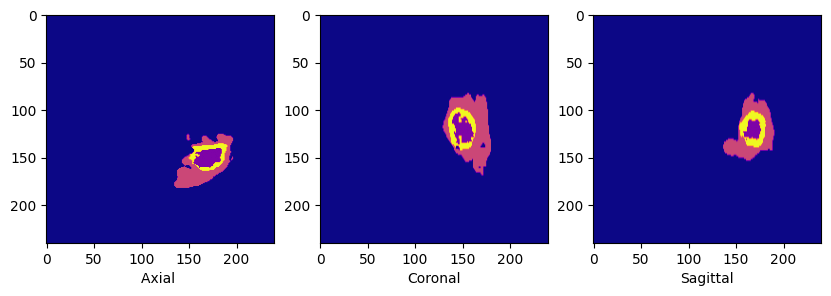
\includegraphics[height=2in]{Experimental/Chapter2Figs/tumour_regions.jpg}
    \else
      \includegraphics[bb = 92 86 545 742, height=6in]{tumour_region}
    \fi
    \caption{Tumour regions (in the axial, coronal, saggital directions). The different colours depict the multiclass pixel labels}
    \label{tumour_region}
  \end{center}
\end{figure}
As can be seen, the tumour regions are distinctly prominent in all the 3 directional axes. These mask categories are independent of the MRI modality. They show the ground-truth labels of the pixels that depict the tumour tissue. 

\subsection{Methylated and Non-methylated tumours}
%\vspace*{1mm}
According to the discussed background of the problem, the methylation status of the MGMT gene can be correlated with biomarkers in the MRI scan. The methylation status can be informally judged by looking at the distribution of the tumour pixel categories, and in the way the tumour region is spread out. 

%\vspace*{2mm}


\begin{figure}[H]
  \begin{center}
    \leavevmode
    \ifpdf
      \includegraphics[height=2.9in]{Experimental/Chapter2Figs/methylated_unmethylated.jpg}
    \else
      \includegraphics[bb = 92 86 545 742, height=6in]{methylated_unmethylated}
    \fi
    \caption{(A) Unmethylated tumours and (B) Methylated tumours}
    \label{methylated_unmethylated}
  \end{center}
\end{figure}

The unmethylated tumour exmaples in (A) have a less-defined tumour core region, and although the invaded tissue extent is large, the necrosis of the core is subdued. Whereas in methylated samples (B), the tumour core is starkly prominent and the tumour growth is visible from inside-out.
\vspace*{2mm}

The methylation classification of the tumour is challenging because the tissue biomarker of the underlying genomic characteristic is not directly inferrable. In the methylation ground-truth labels provided as training data, a 10\% benchmark across the gene sites was considered for the binary classification. Since the MRI scans can have varying levels of carninoma and the MGMT methylation percentage can vary, therefore there remains some sort of ambiguity in the visible differences. 

\section{Model architectures}

Various model architectures were experimented for the segmentation and classification tasks. All the models that were based on 2D Convolutional Neural Networks (CNN) and the input data had multiple channels based on the requirement.

\subsection{UNet 2D }
\vspace*{2mm}
U-Net was introduced by \cite{Unet} for highly accurate biomedical semantic image segmentation. It gained popularity because it required less number of training samples. 
\vspace*{2mm}

UNet is based upon the encoder-decoder model of deep CNN archictecture and incorporates an encoder block, skip connections and a decoder block. It combines feature extraction and feature localization strategies. 

\begin{enumerate}
    \item \textbf{Encoder block:} Encoder captures the most relevant information in the input image into a lower-dimesnional space, by extracting the most definitive features. It uses a series of convolution, pooling and fully-connected layers to arrive at a compact representation. 
    \item \textbf{Decoder Block}: Decoder block is the exact opposite of the encoder operation. By using the compact feature representation, it reconstructs the image by using deconvolutional and upsampling operations which increase the image dimensionality.
    \item \textbf{Skip connections}: This step is crucial for preserving the locational or spatial information of the image. In U-Net, skip connections are used to pass information from earlier convolutional layers to the deconvolution layers. What is passed is the location of the feature extracted by convolutional layers. This is done by concatenating the last layer in the convolutional block with the first layer of the opposite deconvolutional block.
\end{enumerate}

The UNet architecture is symmetrical and the dimensions of the opposite layers/blocks will be the same. If we input a (X,Y) dimensional 2D image which is to be semantically segmented to 4 classes, then the output image will be (X,Y,4) in the categorical data format.

\subsection{Multi-task-learning (MTL) model}
\vspace*{2mm}
A novel Multi-task-learning model was developed from an UNet adaptation. Multi-task-learning models refers to networks which are optimized for more than one task, and they simultaneously train the network parameters for all the tasks. By sharing representations between the related tasks, it avoids overfitting and enables the model to learn better.
\vspace*{2mm}

In our problem statement, the \textbf{segmentation} and \textbf{classification} tasks are related to one another and can be learnt jointly. We employ \textbf{Hard parameter sharing} in which there are task-specific individual layers and shared layers. Shared layers have to learn parameters that fit both the given tasks. The model back-propagates along both the individual and the shared layers.

\begin{figure}[H]
  \begin{center}
    \leavevmode
    \ifpdf
      \includegraphics[height=2.1in]{Experimental/Chapter2Figs/MTL_shared.png}
    \else
      \includegraphics[bb = 92 86 545 742, height=6in]{MTL_shared}
    \fi
    \caption{A general MTL model showing shared and task-specific layers}
    \label{MTL_shared}
  \end{center}
\end{figure}

The semantic segmentation model of UNet was adapted into an MTL model by adding the \textbf{classification branch}. The classification branch utilizes the compact feature representations from the lowest 3 blocks of the UNet (one from encoder, one from decoder and the bridge layer). Since these 3 blocks have outputs of different dimensionality, we use a \textbf{Global Average Pooling (GAP)} layer after each, which scales down the input dimensions of \textbf{(X, Y, Z)} to \textbf{(1, 1, Z)} by doing a average operation. The reduced image features are then joined by a concatenation layer which is passed to a Fully-connected layer (with Softmax activation function) to get the final binary classification. For any test image, a two-tuple output is given by the model. The 1st output is the segmentation mask, and the 2nd output is the probability of the classification label (methylated/ unmethylated). 
\begin{center}
    $L_{joint} = \lambda L_{cls} + (1-\lambda) L_{seg}$
\end{center}
%\vspace*{1mm}
The loss function of an MTL model is jointly given by the loss of the classification $L_{cls}$ and the loss of segmentation $L_{seg}$, weighted by a parameter $\lambda$. By changing the value of $\lambda$ we can give more weightage to either of the tasks.
\vspace*{4mm}

\begin{figure}[H]
  \begin{center}
    \leavevmode
    \ifpdf
      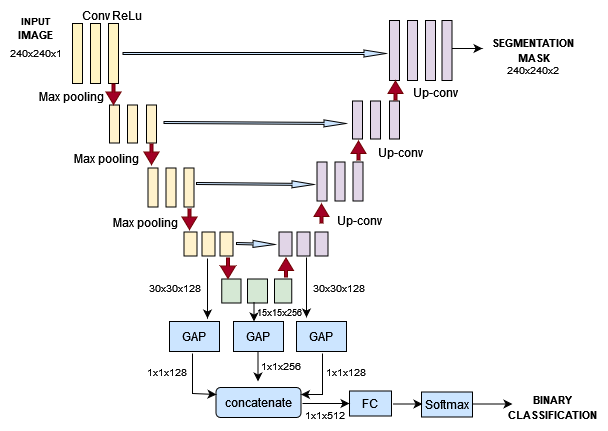
\includegraphics[height=4in]{Experimental/Chapter2Figs/MTL.png}
    \else
      \includegraphics[bb = 92 86 545 742, height=6in]{MTL_fig}
    \fi
    \caption{Our U-Net adapted MTL model}
    \label{MTL_fig}
  \end{center}
\end{figure}


\subsection{ResNet18 and ResNet34}
\vspace*{3mm}
A new category of deep networks called \textbf{Residual networks (ResNet)} was introduced in \cite{resnet}. The layers are reformulated to learn residual functions with reference to the layer inputs, instead of learning unreferenced functions. These ResNets are easier to optimize, and can gain accuracy from considerably increased depth. By using \textbf{'skip connections'} periodically in the model architecture,  activations of a layer are connected to further layers by skipping some layers in between, thus forming a \textbf{'Residual Block'}. Identity shortcut connections add neither extra parameter nor computational complexity. The entire network can still be trained with back propagation.

%\vspace*{1mm}

\begin{figure}[H]
  \begin{center}
    \leavevmode
    \ifpdf
      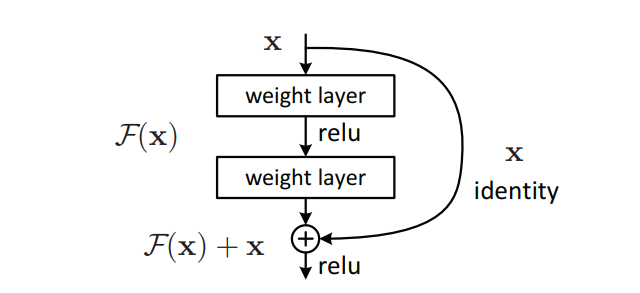
\includegraphics[height=2in]{Experimental/Chapter2Figs/residual_block.PNG}
    \else
      \includegraphics[bb = 92 86 545 742, height=2.5in]{Residual}
    \fi
    \caption{A simple Residual Block (cited from \cite{resnet})}
    \label{Residual}
  \end{center}
\end{figure}

ResNet uses a network architecture inspired by VGG-19 (\cite{vcg19}) in which shortcut connections are added. On the ImageNet dataset,  the authors of the paper uses a 152-layers ResNet, which is 8 times more deep than VGG19 but still have less parameters. In general, \textbf{ResNet18} and \textbf{ResNet34} are used for smaller classification tasks which are 18 layers and 34 layers deep respectively.


\subsection{EfficientNet}
\vspace*{3mm}
A new family of models called EfficientNet was introduced in \cite{effnet}. The EfficientNet architecture uniformly scales all dimensions of depth/width/resolution using a compound coefficient (\textbf{model scaling}). The EfficientNet scaling method uniformly scales network width, depth, and resolution with a set of fixed scaling coefficients, rather than using arbitrary scaling factors.
\vspace*{3mm}

The baseline model \textbf{EfficientNet B0} is based on the inverted bottleneck residual blocks that was demonstrated in MnasNet (\cite{mnasnet}), in addition to the squeeze-and-excitation blocks. The building block of this architecture is the mobile inverted bottleneck MBConv  (inverted residual block) with an additional Squeeze-and-Excitation block. Using compound scaling, \textbf{ EfficientNet B1} to \textbf{EfficientNet B7} are developed, where the number of model parameters increase exponentially, but give higher accuracy. 


% ------------------------------------------------------------------------

%%% Local Variables: 
%%% mode: latex
%%% TeX-master: "../thesis"
%%% End: 
